\section{Methodology}
\ap{2.5 Pages for: Methodology}

%What is our verification approach? --> quick overview on the general idea and the methodology
To address the limitations of current verification approaches, as illustrated by the examples presented above, we propose our novel verification method. Our approach is based on dynamic program analysis in form of mutation-based fuzzing in combination with reinforcement learning techniques. Furthermore, we provide a language for easily expressing intended P4 program behaviour, so properties to be verified by the system. Figure .. presents an overview of the verification methodology. First the user specifies behavioural properties of the program to be verified. Together with the configuration of the control plane, it is the input for the Reward System, providing the baseline for the verification. The reinforcement learning Agent defines the mutation actions to be applied for each individual packet, that will be generated by the packet generator. For that, it is using the information returned by the monitoring unit, about the processing applied to the packets.

The following provides further details on the language defined, as well as the fuzzing and reinforcement learning approach.

\begin{figure*}
  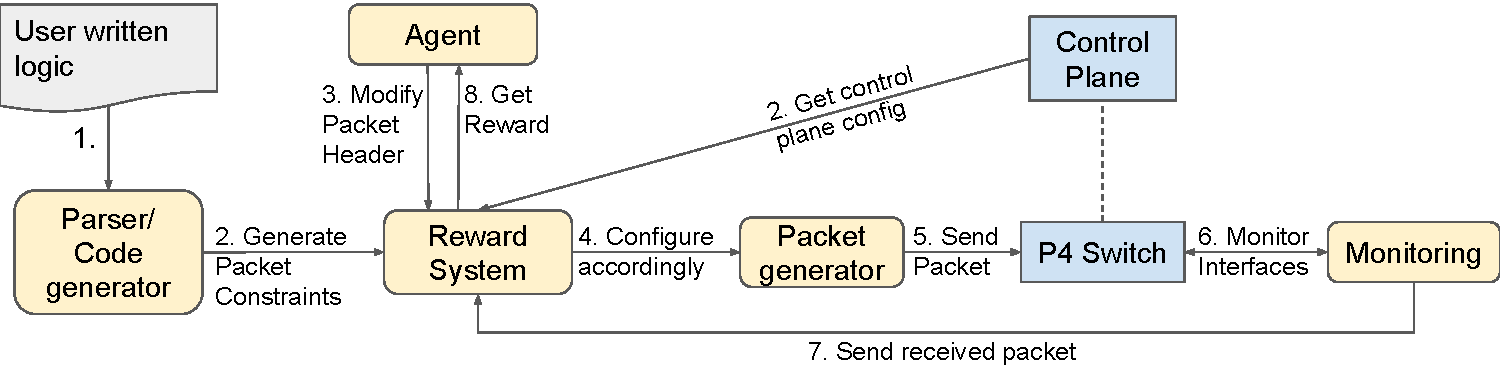
\includegraphics[width=\textwidth]{figures/methodology_v4.pdf}
  \caption{Methodology \kh{you referred to the connection P4 switch <-> control plane right? Or control plane <-> Reward system?} \ap{I mean make a line-shaped like 7. Send received packet and not diagonal}}
\end{figure*}

\subsection{Program Behavior Description Language}
% user friendly interface 
\kh{Didnt really know how to call the section on the language we defined, so feel free to edit the title of this section}

A P4 program alone does not fully describe the intended behaviour of a data plane device, as it is envisioned by the programmer. The implementation of the control plane has high importance for the behaviour of the P4 program. In addition to that, target dependent components in the packet processing pipeline, can influence the packet processing as well. So together with the goal of automating the P4 program verification process, it is inevitable to provide a language specifically designed for expressing P4 program behavioural properties. 
As a result, we propose \lang, the program behavior description language. One of the major design goals of \lang was to provide a user friendly interface for \system. To achieve this, the structure for expressing P4 program properties is kept simple. Each property to be checked is described as tuple in an if-then-else fashion. The user specifies conditions the packet has to fulfill at ingress of the switch (if), together with conditions the expected packet egress should fulfill at egress (then). Optionally the user can describe alternative conditions in case the conditions in the "then" branch are not fulfilled at egress (else). 

Figure .. gives an overview on the grammar and constructs defined in \lang. The grammar allows common boolean expressions and relational operators as they can be found in many programming languages like C, Java or Python, to ease the work for the programmer. Furthermore it comprises the primitive methods \textit{isCorrect()} and \textit{table\_val()}. The \textit{isCorrect()} method is used to denote the need for verifying a header checksum. The \textit{table\_val()} method will check if the correct value has been placed as expected by the current control plane configuration, e.g. for exchanging the destination mac address during layer 3 processing.

% further description, examples and figure still missing

%\begin{itemize}
 %   \item describe the language/purpose of it/why do we need the language?
  %  \item design process aimed at providing user friendly interface --> make it easy for programmers to use the language, if-then-else structure
   % \item explain the grammar/syntax and show an example
    %\item \kh{maybe small figure similar to p4v description on GCL?}
    %\item explain workflow of defining and generating properties for verification
%\end{itemize}

\subsection{Machine Learning Assisted Fuzzing}
% automation
% describe the need & thought process


\begin{itemize}
    \item dynamic testing and fuzzing
    \item mutation based fuzzing
    \item how to interpret mutation based fuzzing as game to be used with reinforcement learning, similarity feedback + reward system
    \item Packet generation and monitoring of the interfaces
\end{itemize}

\ap{Think about a simple language/constructs or utility, we provide to users for specifying properties that we would like to verify. That will have a better impact. }
\begin{itemize}
    \item explain the idea of combining mutation based fuzzing with the reinforcement learning:
    \item interpreting mutation based fuzzing as game to be able to apply reinforcement learning methods
    \item connect mutation based fuzzing as game for reinforcement learning, with verification through sending packets with mutated header values to test for/ trigger bugs by comparing the packet as it was sent to the ingress port of the switch with the resulting processed packet at egress of the switch and applying rules for checking e.g. protocol compliant processing.
    \item use this result as input for reward function, providing the feedback used to train the reinforcement learning model
\end{itemize}